Nella sezione \ref{Preliminari} abbiamo visto come l'ipotesi di varietà taut ci permette di dire, se le orbite di una certa funzione non sono relativamente compatte, che la successione delle iterate è compattamente divergente.

Per ottenere un teorema di tipo ``Wolff-Denjoy'', nel caso in cui le iterate siano compattamente divergenti dobbiamo dire due cose: che le iterate convergono uniformemente sui compatti a una funzione a valori nel bordo euclideo, e che in realtà tale funzione è una costante.

La convergenza al bordo uniforme sui compatti è data dalla Proposizione \ref{montel}, supponendo che la varietà sia una sottovarietà tautly embedded di una varietà Kobayashi-iperbolica. Per dire che la funzione limite è costante, invece, ci serviranno delle ipotesi aggiuntive di tipo geometrico: la condizione di visibilità per le simil-geodetiche.

Nel seguito, ricordiamo che data una varietà complessa $X$ abbiamo fissato una metrica hermitiana $\|\cdot\|_X$, che nel caso in cui $X$ sia connessa induce una distanza $d_X$. Se abbiamo delle sottovarietà, fissiamo la metrica sulla varietà ambiente e prendiamo la restrizione sulle sottovarietà, e se la varietà ambiente è $\mathbb{C}^d$ prendiamo la metrica euclidea. Ricordiamo inoltre che, se $X\subseteq Y$ è un sottospazio topologico, abbiamo posto $\partial_YX=\overline{X}\setminus X$.

\begin{defn}
    Sia $X$ una varietà complessa e connessa; fissiamo due costanti $\lambda \ge 1$ e $\kappa \ge 0$. Sia $I\subseteq \mathbb{R}$ un intervallo; una curva $\sigma:I \longrightarrow X$ è detta una \textit{$(\lambda,\kappa)$-simil-geodetica} se
    \begin{enumerate}
        \item per ogni $s,t \in I$ si ha
        \begin{equation} \label{simil-geo1}
            \frac{1}{\lambda}|t-s|-\kappa \le k_X\big(\sigma(s),\sigma(t)\big)\le\lambda|t-s|+\kappa;
        \end{equation}
        \item $\sigma$ è assolutamente continua rispetto a $d_X$ (quindi $\sigma'(t)$ esiste per quasi ogni $t \in I$) e per quasi ogni $t \in I$ si ha
        \begin{equation} \label{simil-geo2}
            K_X\big(\sigma(t);\sigma'(t)\big) \le \lambda.
        \end{equation}
    \end{enumerate}
\end{defn}

\begin{defn} \label{visibility}
    Sia $X$ una sottovarietà complessa e connessa di una varietà complessa $Y$, e fissiamo $\lambda \ge 1$ e $\kappa \ge 0$. Diciamo che $X$ è \textit{$(\lambda,\kappa)$-visibile} se
    \begin{enumerate}
        \item ogni due punti distinti di $X$ possono essere collegati da una $(\lambda,\kappa)$-simil-geodetica;
        \item per ogni coppia di punti $p,q\in\partial_YX$ con $p\not=q$, esistono in $\overline{X}$ due intorni $V$ e $W$, di $p$ e $q$ rispettivamente, con chiusura disgiunta, e un compatto $K$ di $X$ tali che  ogni $(\lambda,\kappa)$-simil-geodetica in $X$ che collega un punto di $V$ a un punto di $W$ interseca $K$.
    \end{enumerate}
\end{defn}

\begin{oss} \label{spscvxisvis}
    Nel caso di un dominio limitato con bordo regolare, l'ipotesi di essere strettamente pseudoconvesso permetteva di concludere la condizione geometrica di Gromov-iperbolicità. Inoltre, in tal caso il dominio è proprio e completo (si veda \cite[Paragraph 3.3]{G}); dunque, ricordando l'Osservazione \ref{lengthspace}, per il teorema di Hopf-Rinow (\cite[Part I, Proposition 3.7]{BH}) è uno spazio geodetico, cioè ogni coppia di punti è collegata da una geodetica. Si può dimostrare che gli spazi Gromov-iperbolici, propri e geodetici sono visibili sia per le geodetiche che per le simil-geodetiche: per le prime si può ragionare come in \cite[Proposition 2.5]{BNT}, usando il fatto che per ogni coppia di punti distinti di $\partial^G X$ esistono due loro intorni disgiunti in $X\cup\partial^GX$ (si veda \cite[Part III, Chapter H, Lemma 3.6]{BH}); per le seconde, segue da \cite[Part III, Chapter H, Theorem 1.7]{BH}.
\end{oss}

Tuttavia, nella sezione \ref{Esempi di domini con visibilità} vedremo esempi di domini che sono visibili per le simil-geodetiche ma che non sono Gromov-iperbolici. Segue dunque che i risultati che andremo a dimostrare sono, in un certo senso, più generali. In particolare, il Teorema \ref{abate_wd} sarà un corollario del teorema che dimostreremo. \\

Le simil-geodetiche sono delle curve che, a meno di costanti moltiplicative e additive, si comportano come le geodetiche, cioè come le curve che minimizzano la lunghezza.
Quello che chiediamo, euristicamente, nella Definizione \ref{visibility} è che, se vogliamo andare da un punto a un altro del bordo con tali curve, allora non possiamo stare arbitrariamente vicini al bordo, ma siamo costretti a ``piegarci'' verso l'interno; in pratica, stiamo chiedendo che ci sia una sorta di curvatura negativa.

\begin{figure}[h!]
    \begin{center}
        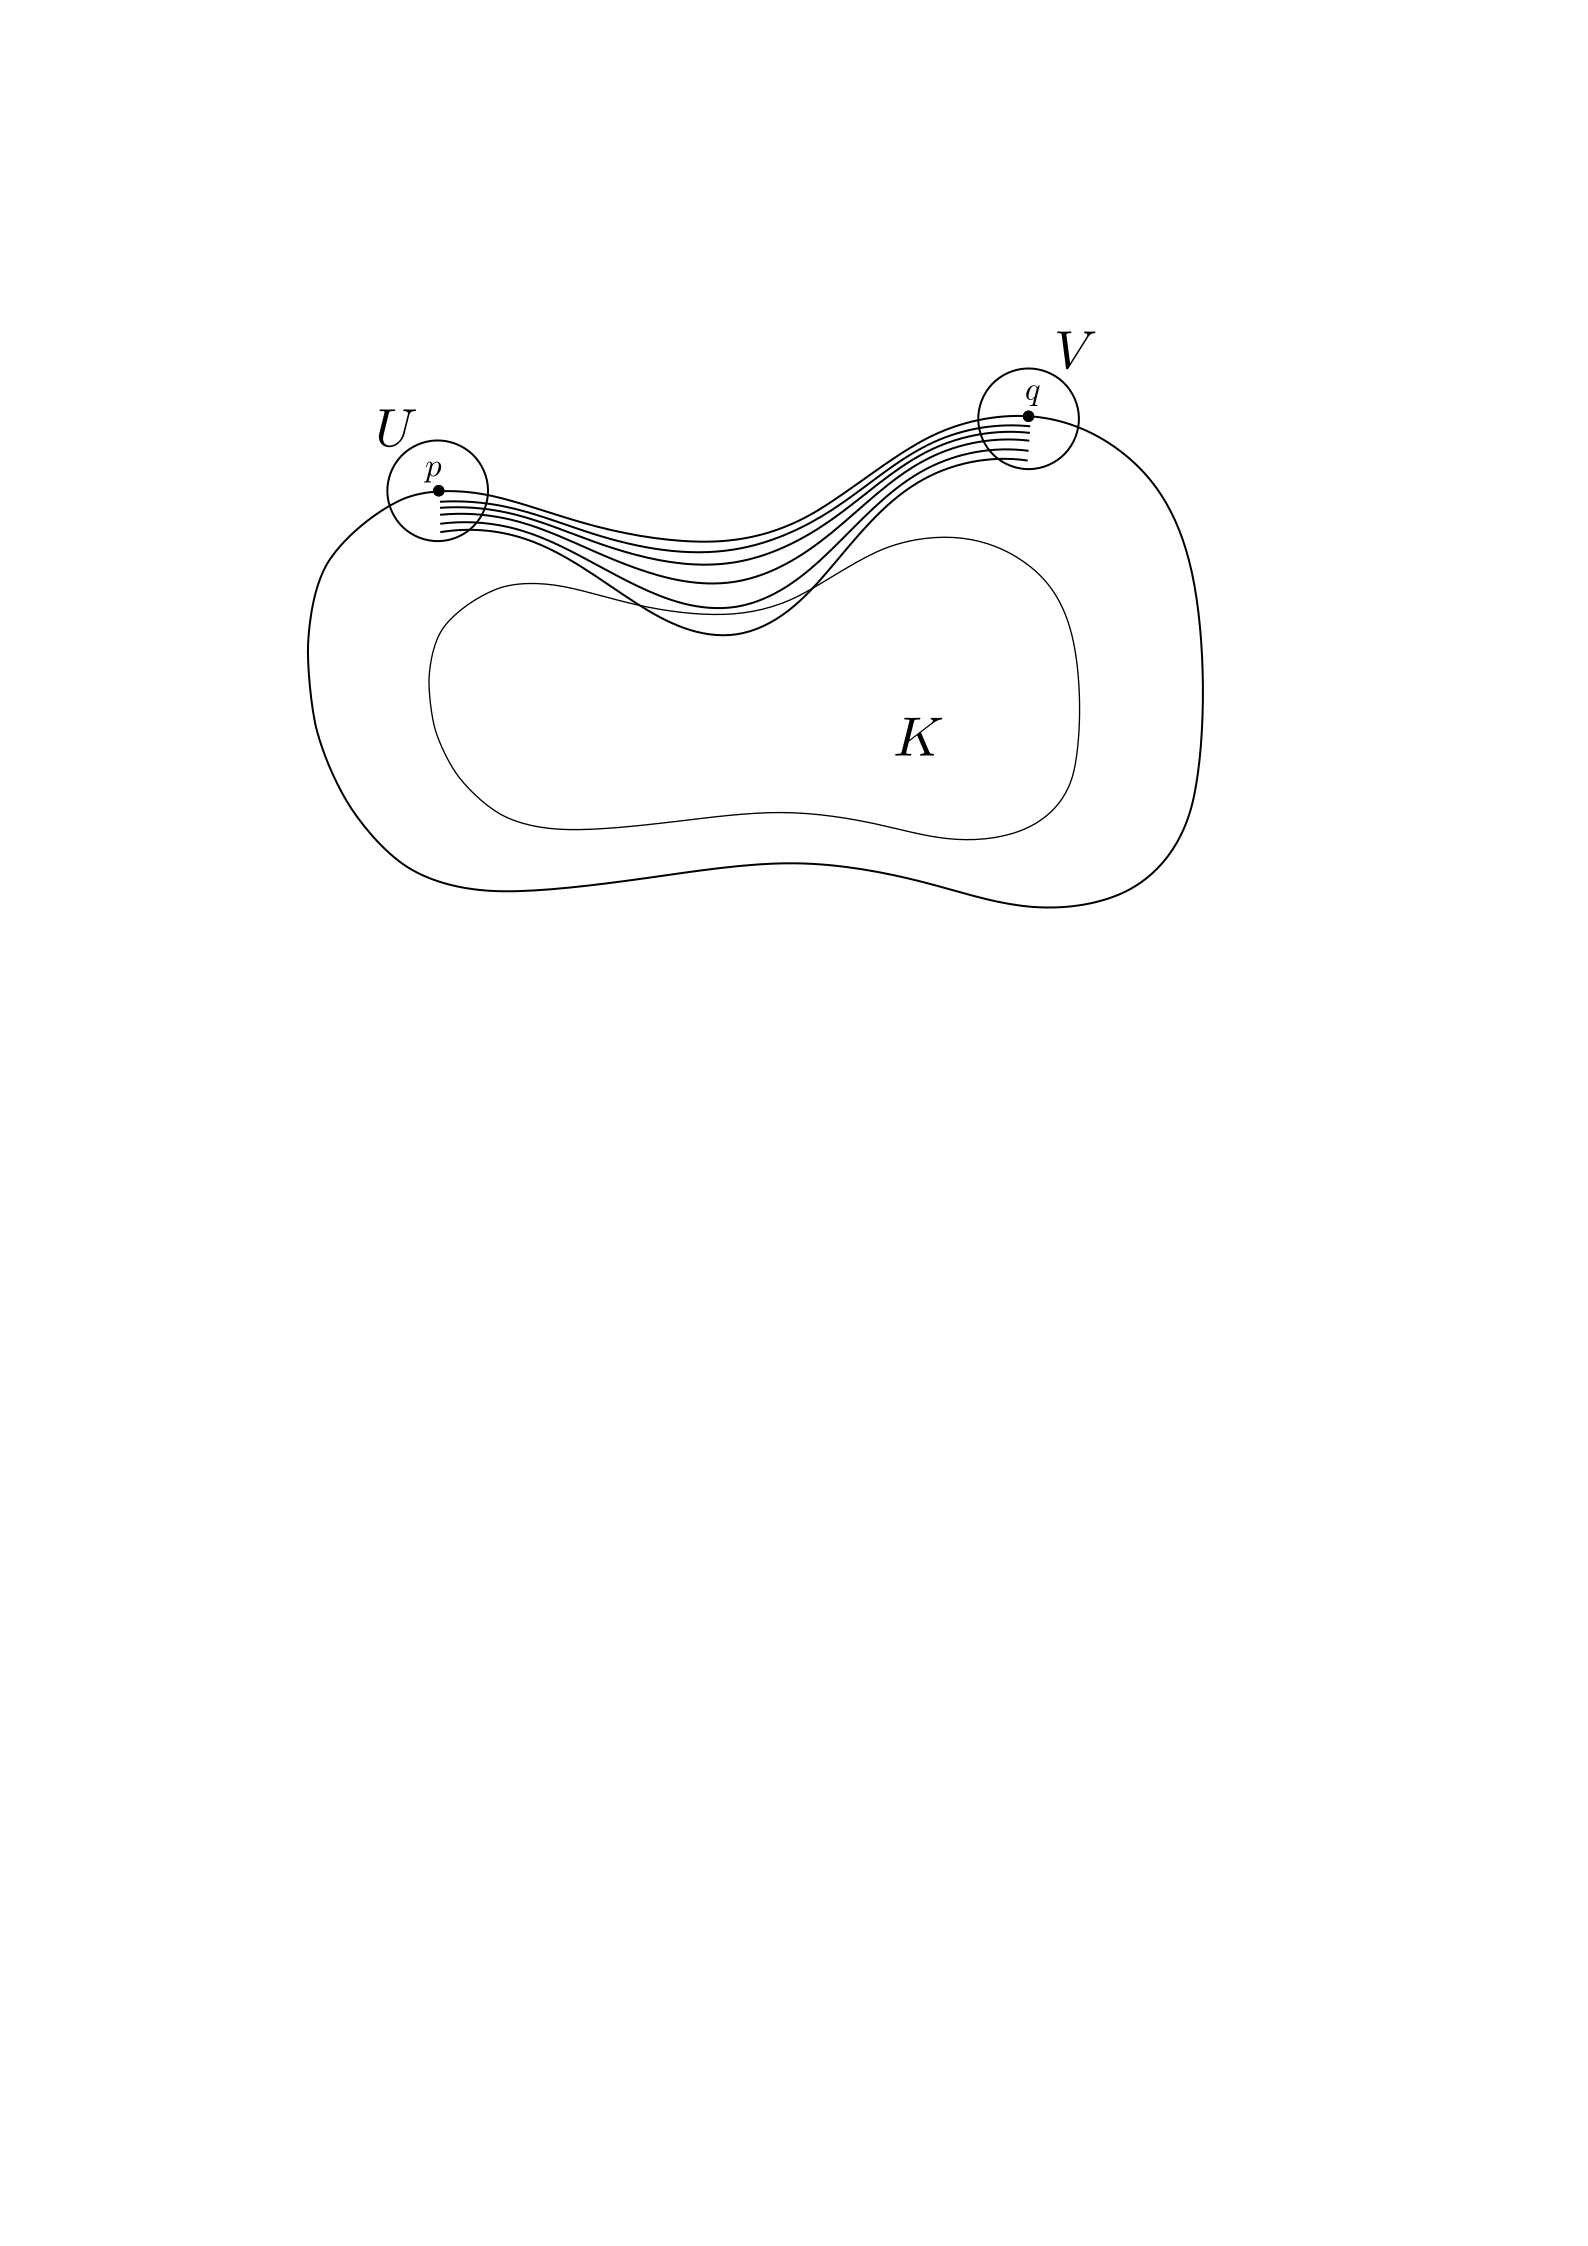
\includegraphics[width=1.05\textwidth, trim=0 18cm 0 5cm]{Immagini/nonvis.png} \\
        \caption{il caso, da noi escluso, in cui le simil-geodetiche da $U$ a $V$ fuggono dai compatti di $X$}
    \end{center}
\end{figure}
\newpage
\begin{figure}[h!]
    \begin{center}
        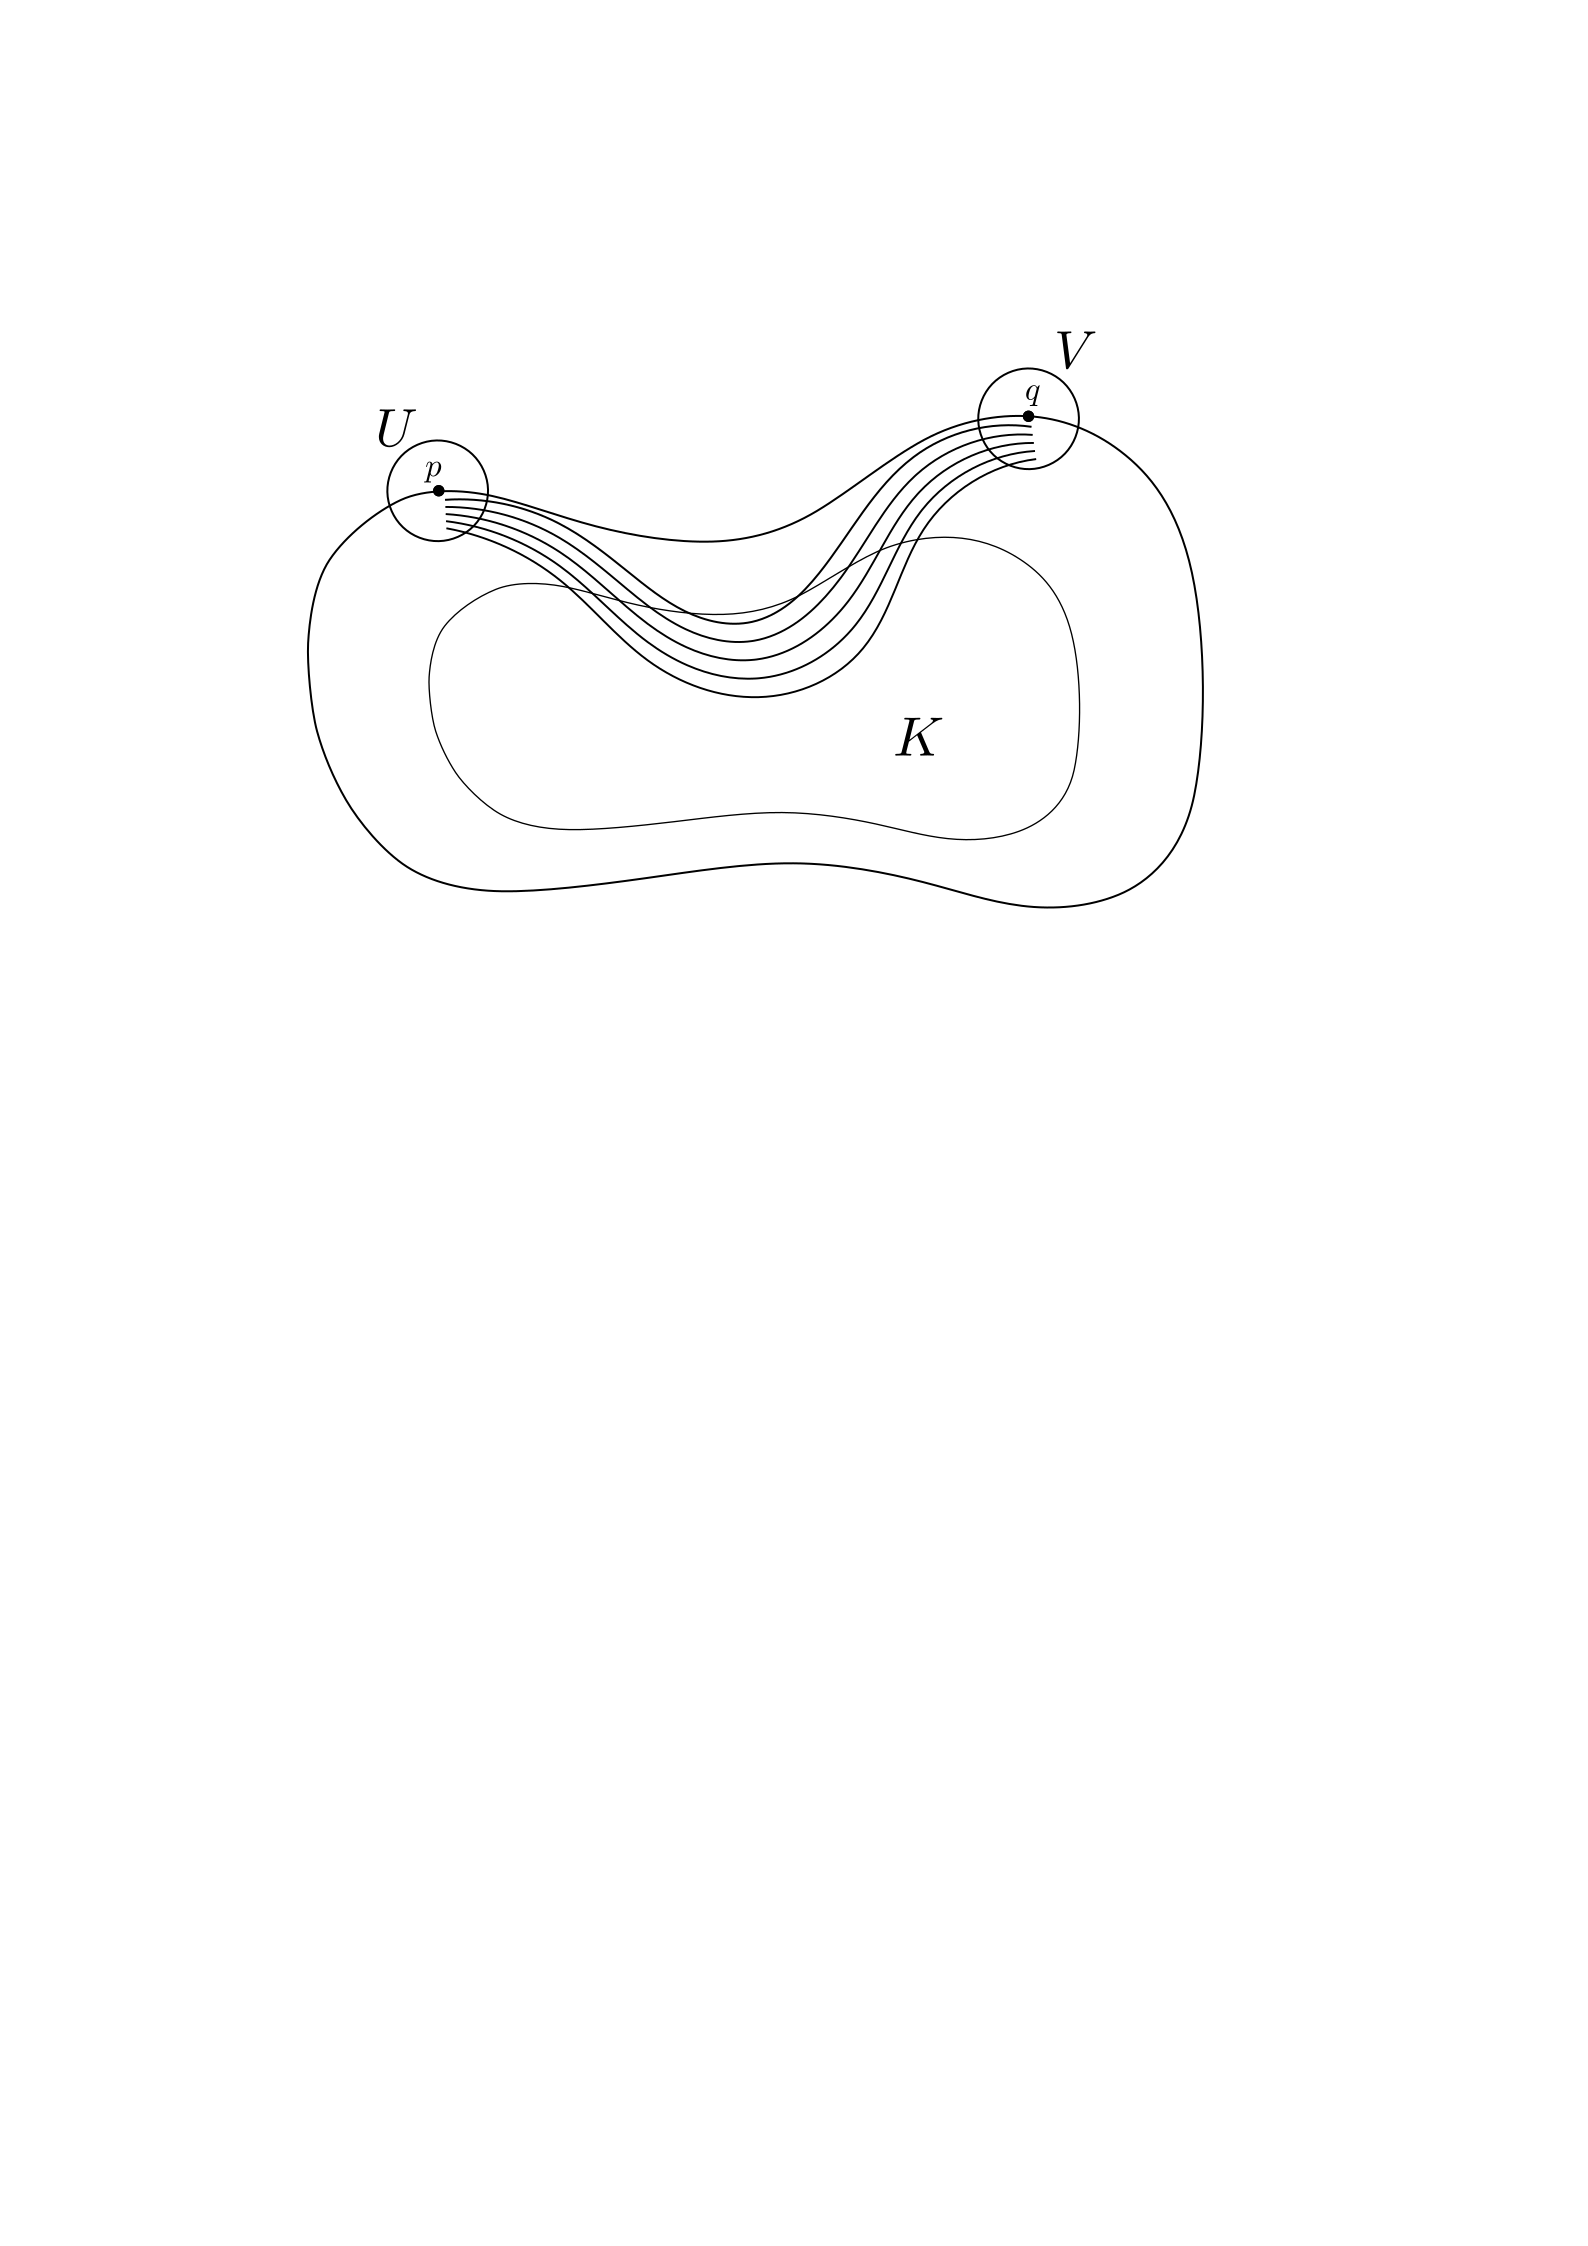
\includegraphics[width=1.05\textwidth, trim=0 18cm 0 5cm]{Immagini/vis2.png} \\
        \caption{sotto ipotesi di visibilità, le simil-geodetiche da $U$ a $V$ devono curvare verso l'interno per intersecare un compatto $K$}
    \end{center}
\end{figure}

\begin{ex}
    Il dominio $\Omega$ definito nell'Esempio \ref{servetaut} è $(\lambda,\kappa)$-visible per ogni $\lambda \ge 1$ e $\kappa \ge 0$. Per vederlo, fissiamo $\lambda$ e $\kappa$ e consideriamo due casi:
    \begin{nlist}
        \item uno dei due punti è l'origine. Allora basta prendere come compatto un qualsiasi insieme della forma $\{r \le |z| \le R\}$ con $0<r<R<1$ e i due intorni aperti sufficientemente piccoli;
        \item i due punti sono entrambi sulla sfera unitaria. Per \cite[Proposition 6]{NTT} è facile vedere che, se la palla unitaria è $(\lambda,\kappa)$-visibile, allora $\Omega$ soddisfa la condizione voluta anche in questo caso. Ma la palla unitaria è limitata, ed è facile vedere che è strettamente pseudoconvessa; quindi, per l'Osservazione \ref{spscvxisvis}, è $(\lambda,\kappa)$-visibile, come voluto.
    \end{nlist}
    Perciò, l'ipotesi che la varietà sia taut è necessaria per ottenere un teorema di tipo ``Wolff-Denjoy'', anche con la condizione di visibilità.
\end{ex}